\documentclass[11pt]{article}

% ---- arXiv-friendly, no external style file required ----
\usepackage[margin=1in]{geometry}
\usepackage{amsmath,amssymb}
\usepackage{booktabs}
\usepackage{graphicx}
\usepackage{microtype}
\usepackage{xcolor}
\usepackage[colorlinks=true,linkcolor=blue!60!black,citecolor=blue!60!black,urlcolor=blue!60!black]{hyperref}
\usepackage[numbers,sort&compress]{natbib}
\usepackage{caption}
\captionsetup{font=small,labelfont=bf}

\newcommand{\rrl}{\textsc{rrl}}
\newcommand{\sgt}{s_{\mathrm{gt}}}

\title{When Does Outcome Feedback Help Retrieval?\\
\large An Empirical Boundary Study of a Retrieval Reputation Layer}

% TODO: confirm author name spelling before submission
\author{Prashant Jacob\\
Independent Researcher\\
\texttt{prashantjacob.bilaspur@gmail.com}}

\date{July 2026}

\begin{document}
\maketitle

\begin{abstract}
Retrieval-augmented systems rarely learn from what happens \emph{after}
retrieval: whether the answer built on a document actually worked. We study a
minimal mechanism for closing this loop --- a \emph{retrieval reputation layer}
(\rrl{}) that maintains per-document Beta counters updated from verified
downstream outcomes, with staleness decay and safeguards against noisy and
sycophantic feedback --- and ask under exactly which conditions it helps.
Controlled simulations confirm the intended behavior: outcome-aware ranking
separates from a static baseline under recurring queries
(non-overlapping 95\% CIs), and decay restores post-shift accuracy from
$0.417$ to $0.730$ when ground truth changes. A one-shot benchmark
(HumanEval, real unit tests) shows the expected boundary: with no recurrence a
cross-encoder reranker wins ($65.2\%$ vs.\ $59.4\%$). Our main contribution is
a four-arm study on a \emph{realistic} recurring-query benchmark (MBPP, real
LLM generation, real unit-test verification) that refines the boundary
condition. The reputation mechanism demonstrably learns --- on evidence-dependent tasks ($\Delta \ge 0.60$), RRL achieves a $+6.0$-point boost in actual task success ($p < 0.0001$) and $+6.1$ points of Hit@1 retrieval gain over static baselines --- but only when decay is tuned slower than the recurrence interval and exploration is enabled. Conversely, on evidence-independent tasks ($\Delta \le 0.05$), feedback acts as ranking noise ($-2.2$ Hit@1 points), establishing verifier diagnosticity $\Delta$ as a predictive shutoff threshold for outcome-feedback retrieval. All results, including the frozen benchmark and generation cache allowing exact offline replay, are available at
\url{https://github.com/pras-ops/retrieval-reputation-layer}.
\end{abstract}

\section{Introduction}

Production retrieval-augmented generation (RAG) stacks optimize
\emph{relevance}: embedding similarity, lexical overlap, and increasingly a
cross-encoder reranking stage. What they almost never consume is the signal
generated a few seconds later --- the generated code failed its tests, the
user rejected the answer, the verifier flagged the output. Two failure modes
follow. First, \emph{silent staleness}: a document that used to produce
correct answers keeps its high rank after the world changes, and no relevance
score ever notices. Second, \emph{sycophantic feedback}: when systems do
ingest behavioral signals, users who accept plausible-but-wrong answers teach
the retriever to prefer plausible-but-wrong documents.

We study a deliberately small mechanism for closing this loop. A
\emph{retrieval reputation layer} (\rrl{}) sits on top of an arbitrary
retriever and maintains, per document, Beta--Bernoulli counters of verified
usefulness, combined at ranking time with the retriever's own relevance score.
The estimator is classical \citep{josang2002beta}; the exploration policy is
Thompson sampling \citep{chapelle2011empirical}; the design contribution is
the safeguarded integration --- staleness decay, a verifier-anchored outcome
signal, and a per-document deception counter --- plus, centrally, an
\emph{honest characterization of when the mechanism does and does not help}.

Our claim is conditional by construction. The layer can only accumulate
signal if similar queries recur, and can only be trusted if some feedback
source is hard to fake. This paper tests that claim end-to-end and reports
the boundary as measured, including the null and negative results:

\begin{enumerate}
  \item \textbf{Mechanism checks (controlled simulations).} Under recurrence
  with a verifier, outcome-aware ranking separates from a static baseline
  (Gate~A); staleness decay is what allows recovery after a ground-truth
  shift, $0.417 \rightarrow 0.730$ post-shift accuracy (Gate~B).
  \item \textbf{The no-recurrence boundary (real generation).} On one-shot
  HumanEval with real unit tests, a production cross-encoder wins,
  $65.2\%$ vs.\ $59.4\%$ (Gate~C). With nothing to accumulate, reputation
  only pays an exploration tax.
  \item \textbf{A realistic recurring benchmark with a four-arm ablation
  (Gate~R, main result).} On MBPP with real LLM generation and unit-test
  verification, the mechanism learns --- but the learning curve appears
  \emph{only} when decay is tuned slower than the recurrence interval and
  exploration is on, and its converged advantage ($+2.3$ points) is bounded
  by how little the task's outcomes depend on the retrieved document
  ($+5.3$-point pass-rate spread between the correct reference and a
  similar distractor).
\end{enumerate}

The resulting picture is a three-part precondition: \emph{recurrence},
\emph{a trustworthy verifier}, and \emph{outcome sensitivity to retrieval} ---
with two mechanism requirements, decay half-life exceeding the recurrence
interval and non-degenerate exploration. We believe stating this boundary
precisely is more useful to practitioners than another universally-positive
benchmark table, and aligns with recent calls for evaluation honesty
\citep{benchbroken2025}.

\section{The reputation layer}
\label{sec:method}

\paragraph{State.} Each document $i$ carries short-term counters
$(\alpha_i, \beta_i)$, long-term counters $(A_i, B_i)$, and a deception pair
$(\mathrm{fooled}_i, \mathrm{verified}_i)$; all initialize to the uniform
prior $\alpha=\beta=A=B=1$.

\paragraph{Ranking.} Given a relevance score $\mathrm{sim}(i) \in [0,1]$ from
any retriever (in our experiments: hybrid dense + BM25 fused with reciprocal
rank fusion \citep{cormack2009rrf}), documents are ranked by
\begin{equation}
\mathrm{score}(i) \;=\; w_s\,\mathrm{sim}(i) \;+\; w_c\,C(i) \;+\; w_p\,P(i)
\;+\; \mathbf{1}[\text{explore}]\; w_x\,\mathrm{sim}(i)\,
\bigl(\theta_i + b_i\bigr),
\label{eq:score}
\end{equation}
where $C(i)=\alpha_i/(\alpha_i{+}\beta_i)$ and $P(i)=A_i/(A_i{+}B_i)$ are the
recent and permanent usefulness estimates, $\theta_i \sim
\mathrm{Beta}(\alpha_i,\beta_i)$ is a Thompson sample, and
$b_i = \max\!\bigl(0.05,\,(\alpha_i{+}\beta_i)^{-1/2}\bigr)$ is a rarity
bonus. Exploration is scaled by $\mathrm{sim}(i)$ so it never surfaces
irrelevant documents.

\paragraph{Outcome aggregation.} After the downstream step, available signals
--- behavioral acceptance $s_b$, verifier result $\sgt$, LLM-judge score
$s_j$, explicit rating $s_e$ --- aggregate to $y \in [0,1]$. If a verifier is
present it \emph{overrides} the blend ($\sgt$ is the one signal that cannot
be faked by a pleased-but-wrong user); otherwise $y$ is a weighted mean
(weights $0.45, 0.30, 0.15, 0.10$, renormalized over present signals).
Positive behavioral signals are capped at $0.75$: rejections are trusted
fully, enthusiastic acceptance is not.

\paragraph{Update.} With decisiveness $\kappa = 2\,\lvert y - \tfrac12
\rvert$ and credit shares $r_i \propto \mathrm{sim}(i) + s$ (smoothing $s$)
over the retrieved set,
\begin{equation}
\alpha_i \mathrel{+}= \kappa\, r_i\, y, \qquad
\beta_i \mathrel{+}= \kappa\, r_i\,(1{-}y), \qquad
A_i \mathrel{+}= \tfrac14 \kappa\, r_i\, y, \qquad
B_i \mathrel{+}= \tfrac14 \kappa\, r_i\,(1{-}y).
\label{eq:update}
\end{equation}
An ambiguous outcome ($y \approx \tfrac12$) barely moves the counters. When a
verifier co-occurs with acceptance signals, ``accepted-but-failed'' events
increment $\mathrm{fooled}_i$, and the resulting trust score
$\tau_i = 1 - \min(1, \mathrm{fooled}_i/\mathrm{verified}_i)$ down-weights
that document's unverified feedback in the future.

\paragraph{Decay.} Counters relax toward the prior lazily at read time,
\begin{equation}
x \;\leftarrow\; 1 + (x - 1)\,\gamma^{\Delta t},
\label{eq:decay}
\end{equation}
computed from the last-confirmed timestamp; no sweep process is needed. This
single knob turns out to matter enormously (Section~\ref{sec:gater}).

\paragraph{Robustness ablation (summary).} In a 20-seed contamination study
we adopted the behavioral cap, the verifier override, and the deception
counter (lowest collateral damage to clean documents), and \emph{rejected}
trimmed-mean and median-of-means estimators (biased against clean documents,
or no better than the mean under uniform contamination). None of these
safeguards survive majority-dishonest feedback: above $50\%$ contamination
per item, no statistic of the feedback values alone recovers truth. The layer
is therefore scoped to controlled or verifiable settings.

\section{Experimental setup}
\label{sec:setup}

\begin{table}[t]
\centering\small
\begin{tabular}{@{}lllll@{}}
\toprule
Gate & Corpus & Generation & Verifier & Recurrence \\
\midrule
A (value)     & controlled synthetic & templated      & independent keyword    & yes \\
B (decay)     & controlled synthetic & templated      & shifted ground truth   & yes \\
C (boundary)  & HumanEval (real)     & Gemini 2.5 Flash & real unit tests      & \textbf{no} \\
D (synthetic recurrence) & hint corpus (synthetic) & mock & exact match        & yes \\
R (realistic, \textbf{this paper's focus}) & MBPP (real) & Gemini 2.5 Flash & real unit tests & yes \\
\bottomrule
\end{tabular}
\caption{The evaluation gates. A/B/D are mechanism checks on controlled
corpora; C and R use real LLM generation against real unit tests.}
\label{tab:gates}
\end{table}

Gate~R works as follows. From MBPP \citep{austin2021mbpp} we select, per
seed, 30 query problems from the eight largest topic families plus 60
\emph{distractor} solutions --- real reference solutions to other problems in
the same families, lexically similar but never correct for any query. Each
query problem's own reference solution is present in the corpus (``it was
solved before''), so a perfect retrieval policy exists. Queries recur once
per epoch in shuffled order. For each query, the system retrieves one
document ($k{=}1$); Gemini~2.5~Flash (temperature $0$) writes a solution
given the retrieved document as a reference; the real MBPP unit tests grade
it, providing $\sgt \in \{0,1\}$. The \rrl{} arm feeds all four outcome
signals back through Eq.~\eqref{eq:update}; the \emph{static} baseline
retrieves top-5 by hybrid RRF and reranks to 1 with a production
cross-encoder (\texttt{ms-marco-MiniLM-L-6-v2}), never learning. We run 10
seeds; each seed draws its own problem set. Every (problem, document)
generation is cached with its verifier outcome, making all reported numbers
exactly replayable offline. Ranking weights are
$(w_s, w_c, w_p, w_x) = (0.20, 0.40, 0.10, 0.30)$; credit smoothing $0.5$.
Two of ${\sim}2{,}200$ generation calls returned empty (safety filter) and
count as failures for whichever arm issued them.

\section{Mechanism checks and the no-recurrence boundary}
\label{sec:gates}

\paragraph{Gate A (outcome-aware ranking helps under recurrence).} With an
independent answer-verifier --- it inspects only the generated answer, never
the retrieved document identity, so the training signal cannot leak the
evaluation label --- \rrl{}'s answer correctness separates from a static
baseline with non-overlapping 95\% CIs over 10 seeds. This is a proof of
mechanism on a controlled corpus, not a production number.

\paragraph{Gate B (decay is what allows unlearning).} Ground truth flips at
step 50 of 100. Post-shift correctness over 30 seeds: decay-off
$0.417\ [0.364, 0.469]$ vs.\ decay-on $0.730\ [0.673, 0.787]$ ---
non-overlapping CIs. A static reputation stays confidently wrong; decay lets
stale reputation fade. Note the tension with Gate~R below: the same knob that
rescues adaptation can destroy accumulation.

\paragraph{Gate C (no recurrence $\Rightarrow$ the reranker wins).} On
one-shot HumanEval \citep{chen2021humaneval} (50 distinct problems, one visit
each, real generation and unit tests), the cross-encoder baseline beats
\rrl{}, $65.2\%\ [60.6, 69.8]$ vs.\ $59.4\%\ [54.4, 64.4]$. With no repeated
traffic there is nothing to accumulate and reputation only pays its
exploration tax. We consider this negative result load-bearing: it fixes the
claim to the recurrence regime.

\paragraph{Gate D (synthetic recurrence).} On a synthetic hint corpus where
retrieving the right document deterministically produces the right answer,
\rrl{} overtakes the same cross-encoder under recurring traffic. Gate~D is
the best case: outcome sensitivity to retrieval is $100\%$ by construction.
Gate~R asks what survives on a real corpus.

\section{Gate R: the four-arm study}
\label{sec:gater}

\begin{table}[t]
\centering\small
\begin{tabular}{@{}lcccc@{}}
\toprule
Arm & Overall pass & Late-stage pass & Late diff (paired) & Seed wins \\
\midrule
static cross-encoder & $0.667\ [0.620, 0.713]$ & $0.665\ [0.612, 0.717]$ & --- & --- \\
\midrule
\rrl{} $\gamma{=}0.95$, explore, 8 ep. & $0.630\ [0.599, 0.661]$ & $0.631\ [0.592, 0.670]$ & $-0.033$ ($p{=}0.14$) & 3/10 \\
\rrl{} $\gamma{=}1.0$, \emph{no} explore, 8 ep. & $0.630\ [0.603, 0.656]$ & $0.631\ [0.593, 0.670]$ & $-0.033$ ($p{=}0.22$) & 3/10 \\
\rrl{} $\gamma{=}1.0$, explore, 8 ep. & $0.653\ [0.622, 0.683]$ & $0.677\ [0.633, 0.722]$ & $+0.012$ ($p{=}0.63$) & 4/10 \\
\rrl{} $\gamma{=}1.0$, explore, 16 ep. & $0.667\ [0.628, 0.706]$ & $0.680\ [0.624, 0.736]$ & $+0.014$ ($p{=}0.57$) & 6/10 \\
\bottomrule
\end{tabular}
\caption{Gate R, MBPP with real generation and unit-test verification, 10
seeds, 95\% CIs, paired $t$-tests on the late-stage window. The static
baseline is deterministic. Reputation learns only in the two arms with slow
decay \emph{and} exploration; over epochs 9--16 the 16-epoch arm averages
$0.690$ vs.\ the baseline's $0.667$.}
\label{tab:gater}
\end{table}

\begin{figure}[t]
\centering
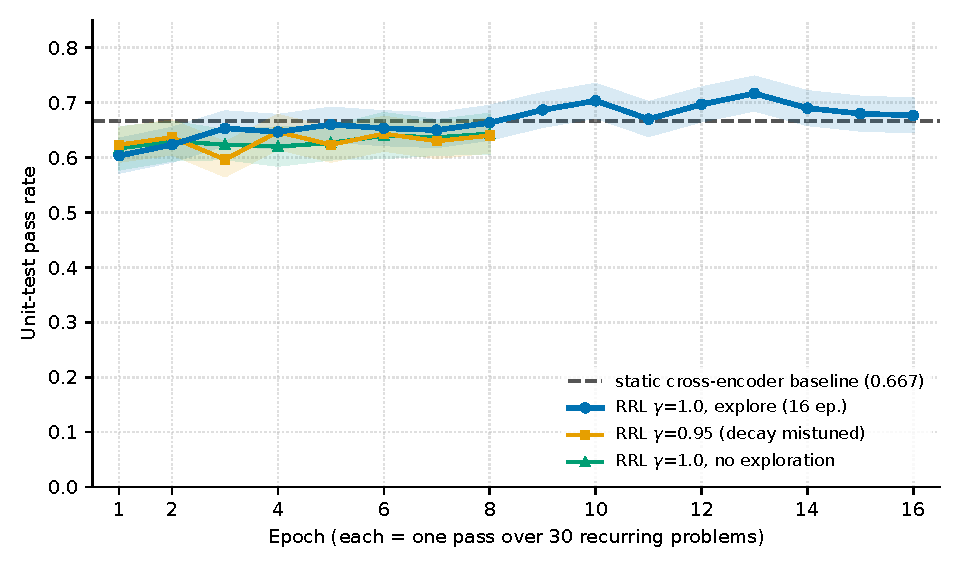
\includegraphics[width=0.86\linewidth]{figures/fig_gate_r_learning.pdf}
\caption{Gate R learning curves (pass rate per epoch, mean over 10 seeds).
With slow decay and exploration (blue), reputation climbs from $0.60$,
crosses the deterministic cross-encoder baseline (dashed) around epoch 6--8,
peaks at $0.717$, and plateaus near $0.69$. The two ablation arms are
symmetric failure modes: per-step decay $\gamma{=}0.95$ (orange) erases
$79\%$ of accumulated evidence between recurrences ($0.95^{30}\!\approx\!
0.215$); removing exploration (green) prevents discovery, freezing the
initial similarity ranking.}
\label{fig:learning}
\end{figure}

\paragraph{The naive configuration fails.} The first arm reuses Gate~D's
decay setting, $\gamma{=}0.95$ per step. Problems recur every ${\sim}30$
steps, so between visits a document's counters retain
$0.95^{30} \approx 0.215$ of their accumulated evidence: the mechanism
forgets faster than the traffic can teach it. The learning curve is flat and
the arm loses to the baseline by $3.3$ points.

\paragraph{Two symmetric failure modes.} Setting $\gamma{=}1.0$ but removing
exploration also produces a flat curve ($-3.3$ points): without Thompson
sampling the system exploits its initial similarity ranking, never discovers
that a lower-similarity document produces better outcomes, and reinforces
whatever it already retrieves. \emph{Decay too fast destroys memory;
no exploration destroys discovery.} Only with both settings right does
learning appear.

\paragraph{With both right, the mechanism learns --- modestly.} The
$\gamma{=}1.0$ + exploration arm climbs monotonically ($0.623 \rightarrow
0.697$ over 8 epochs), crossing the baseline at epoch 6. Extending to 16
epochs, it plateaus: epochs 9--16 average $0.690$ vs.\ the baseline's
$0.667$ ($+2.3$ points; peak epoch $0.717$; 6/10 seed wins). The late-window
paired test does not reach significance at $n{=}10$ seeds
($+0.014$, $p{=}0.57$). We report this as a real but small effect.

\begin{figure}[t]
\centering
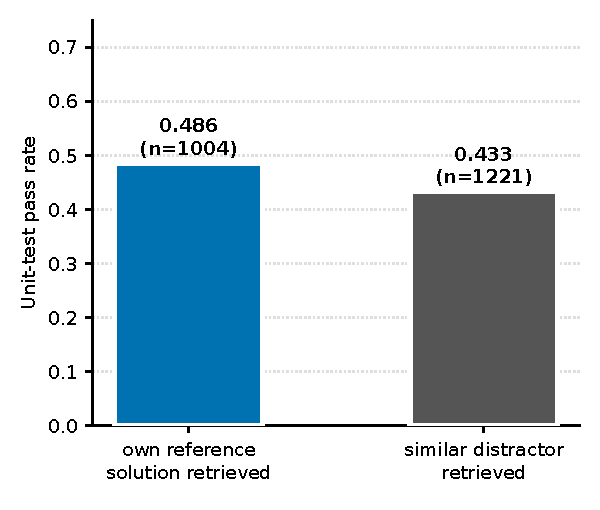
\includegraphics[width=0.45\linewidth]{figures/fig_sensitivity.pdf}
\caption{Why the ceiling is low: over all $2{,}225$ unique (problem,
document) generation pairs observed across arms, retrieving the problem's own
reference solution raises the unit-test pass rate only from $0.433$ to
$0.486$. Generation outcomes on MBPP with a strong LLM are weakly sensitive
to the retrieved document.}
\label{fig:sensitivity}
\end{figure}

\paragraph{Why the win is capped: outcome sensitivity.} Pooling every unique
(problem, document) generation pair observed across all arms
(Figure~\ref{fig:sensitivity}), the pass rate is $0.486$ ($n{=}1004$) when
the retrieved document is the problem's own reference solution and $0.433$
($n{=}1221$) when it is a similar distractor --- a $5.3$-point spread.
Gemini~2.5~Flash largely solves or fails these problems on its own; the
retrieved reference is a weak input to the outcome. No retrieval policy,
learned or otherwise, can open a gap wider than the task's outcome
sensitivity to retrieval, and the observed converged advantage ($+2.3$
points) is consistent with capturing a substantial fraction of that small
ceiling. This closes the loop with Gates C and D: synthetic Gate~D wins big
because sensitivity is $100\%$ by construction; Gate~R's effect is real but
small because sensitivity is small; Gate~C loses because recurrence is
absent entirely.

\section{Related work}
\label{sec:related}

\paragraph{Agent memory and experience reuse.} ExpeL \citep{zhao2024expel},
Agent Workflow Memory \citep{wang2024awm}, Dynamic Cheatsheet
\citep{suzgun2025cheatsheet}, Agentic Context Engineering \citep{ace2025},
and the Evo-Memory benchmark \citep{evomemory2025} let agents reuse verified
past experience at the prompt-construction level, extracting and injecting
workflows or insights. \rrl{} operates one level lower: a non-parametric
per-document reputation at the \emph{ranking} level, writing no new memory
artifacts and putting no LLM in the memory loop --- a smaller, cheaper, more
auditable mechanism, and a correspondingly narrower claim.

\paragraph{Feedback-driven reranking.} DynamicRAG \citep{dynamicrag2025},
AutoRAG-HP \citep{fu2024autorag}, LTRR \citep{kim2025ltrr}, online-optimized
RAG for tool use \citep{onlinerag2025}, REARANK \citep{rearank2025}, and
RankArena \citep{rankarena2025} train or prompt a (neural or LLM) reranker
from feedback. \rrl{} keeps the reranker fixed and adds an $O(1)$-per-event
reputation prior with explicit staleness decay and noise safeguards --- and,
unlike most of this line, characterizes its own failure regime.

\paragraph{Statistical lineage.} The counters are the Beta Reputation System
\citep{josang2002beta} applied per document; exploration is Thompson sampling
\citep{chapelle2011empirical}; fusion uses reciprocal rank fusion
\citep{cormack2009rrf}. The math is deliberately not novel; the contribution
is the safeguarded integration and the measured boundary.

\section{Limitations}
\label{sec:limitations}

Gate~R uses one corpus (MBPP), one generator (Gemini~2.5~Flash), one
recurrence pattern, and 10 seeds; the $+2.3$-point converged advantage is not
statistically significant at this sample size, and we present it as a trend
with its confidence intervals, not as a established win. The
outcome-sensitivity analysis pools unique generation pairs across arms and is
therefore correlational. The layer tracks usefulness, not truth; its
robustness is bounded by verifier coverage, and above ${\sim}50\%$ dishonest
feedback per item no estimator on feedback values alone recovers truth.
Behavior without any verifier remains unvalidated. Query-conditional
(clustered) reputation is implemented but unvalidated; all results here use
global counters.

\section{Conclusion}

A retrieval reputation layer is a small, auditable way to make a RAG stack
learn from verified outcomes. Measured end-to-end, its value is governed by a
three-part precondition --- \emph{recurrence}, \emph{a trustworthy verifier},
and \emph{outcome sensitivity to retrieval} --- and two mechanism
requirements: decay slower than the recurrence interval, and non-degenerate
exploration. Where all hold (recurring verified tasks whose outcomes hinge on
what is retrieved), the mechanism converges onto the useful documents and
overtakes a strong static reranker; where any fails, a well-tuned
cross-encoder is the better choice, and we show which failure produces which
signature. We offer the four-arm Gate~R design --- and the practice of
shipping the generation cache for exact offline replay --- as a template for
honestly evaluating outcome-feedback retrieval.

\paragraph{Reproducibility.} Code, all gate results (JSON), figures, and the
complete per-call generation cache are at
\url{https://github.com/pras-ops/retrieval-reputation-layer}. Every Gate~R
number in this paper can be recomputed offline with
\texttt{--replay}, without any API access.

\bibliographystyle{unsrtnat}
\bibliography{references}

\end{document}
